\chapter{RNA Motifs}
\label{motifs} 
\bibliographystyle{nar}

\section{GNRA tetraloop}
In order to compare our work to that of others on RNA structural motif
localization and discovery, we ask the following questions:
\begin{enumerate}
\item{Can  the geometric rigid-block  description of  base-pairing and
  base-stacking solve the problem of defining RNA structural motifs?}
\item{Can we use quantities derived  from the 3DNA software package to
  make and automatic  search for a known motif,  for example, the GNRA
  tetraloop motif, and perhaps find unknown motifs?}
\end{enumerate}
In the  ROC meeting of May,  2009 a reduced dataset  of RNA structures
found  at:\\  http://docs.google.com/Doc?id=dhrmkfmn\_13ftpbjcgq\\ was
made available  to participants with  the purpose of allowing  them to
search for RNA motifs, which would later be compared between groups.
We  have modestly, and  as of  yet unsuccessfully,  started to  aim at
solving question number  two. Initially we are trying  to identify all
instances of the well known GNRA tetraloop motif in the 23S subunit of
ribosomal  RNA  of  \textit{Thermus Thermophilus},  PDB-ID:1ffk  using
results  from 3DNA  and 3DNA-Parser,  and using  an  automated process
which could be later reproduced  for any desired dataset.  Our hope is
that  these baby  steps  will allow  us  to to  tackle  the whole  ROC
dataset.

\subsection{3DNA-Parser}
We started by using Dr. Yurong Xin's 3DNA-Parser hoping that the
description of the enclosing base pair in the loop, that is, the
sheared G$\cdot$A, would have a characteristic signature.
We found that such is not the case. We know from Major et
al. \cite{lemieux2006} that there should be at least 21 GNRA tetraloops
in the 23S subunit of rRNA. We used the G2696 N2697 R2698 A2699
tetraloop as a seed (as can be seen in Figure 1.1) and found out
that according to Dr. Xin's helical classification the enclosing G is
classified as $S_{hq}$ and A is classified as $H_{e}$. 
\begin{figure}[htbp]
\centering 
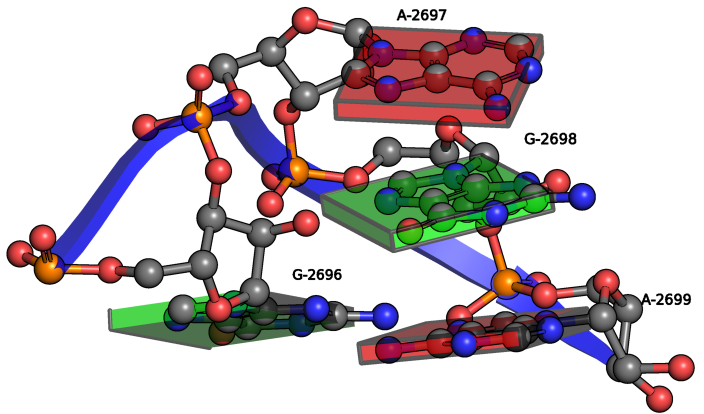
\includegraphics[angle=0, scale=0.5]{Chapter5/gnra.png}
\caption{GNRA Tetraloop from \textit{Thermus Thermophilus} 23S Ribosomal RNA PDB-ID:1ffk.}
\end{figure}
We then searched all such instances for G$\cdot$A base-pairs and we found seven hits,
but none were in fact GNRA tetraloops.

\subsection{Overlap Scores} 
We clustered the overlap values impossing a cutoff of values
of [1-8]. There are many values which are exactly zero (33\%), so,
without the cutoff the zero values "overshadow" the data.
\begin{figure}[htbp]
\centering 
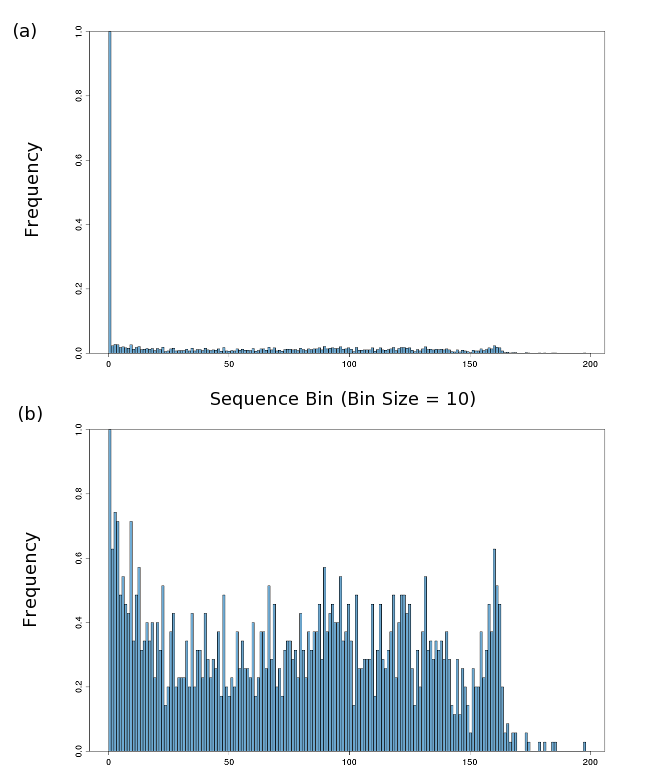
\includegraphics[angle=0, scale=0.8]{Chapter5/histocompare.png}
\caption{Normalized histograms showing the distribution of overlap values in 
the 23S subunit or \textit{Thermus Thermophilus} rRNA, PDB-ID:1jjk. In histogram 
(a) all values are included, but in histogram (b) only values greater than zero are 
included. Notice the high preponderance of zero values, exactly 897 out of a total
of 2705.}
\end{figure}
For this case we obtained a ``good'' dendrogram as seen in Figure 1.2.
\begin{figure}[htbp]
\centering 
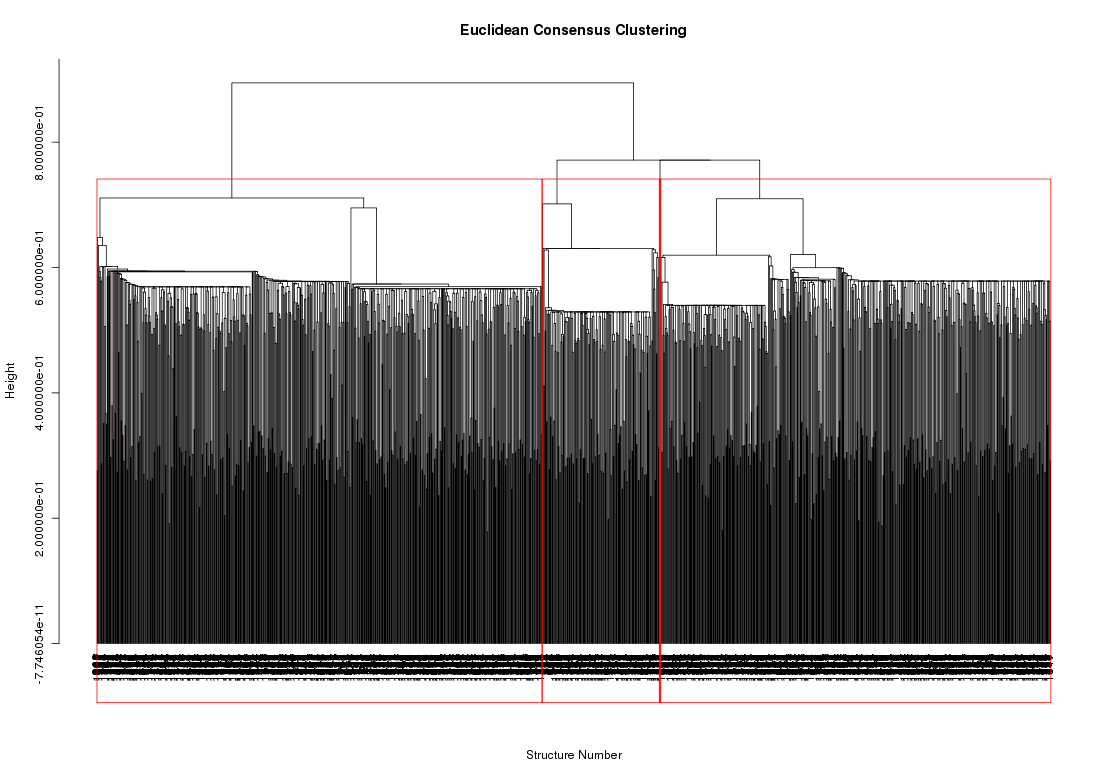
\includegraphics[angle=90, scale=0.6]{Chapter5/eucli_cons.png}
\caption{Dendrogram for consensus clustering of overlap scores in the ribosome.
Zero values filtered out and remaining data normalized.}
\end{figure}

The next step in this analysis will be to find the structures which
correspond to this clusters and superimpose and align them using
Kabsh's algorithm to be able to determine their RMSD's.

Many people start their RNA Motif identification and classification
algorithms by splitting RNA structures into what is helical and what
is not, and then finding interactions between these two groups. We
believe that we could do a similar exercise with 3DNA by using the scalar
product of helical axis vectors and once helical and non-helical
regions are found we might be able to use 3DNA Parser to look for characteristic
interactions.

%\section{Triplets on RNA (comparison to Laing et al.)}


\bibliography{biblio}

